\begin{center}
    \Huge{\textbf{\underline{Chapter 0: Ancient Introduction}}}
\end{center}

\setcounter{section}{0}

\vspace{0.35cm}

\section{Steps Of An Attack}

\vspace{0.25cm}
\begin{center}
    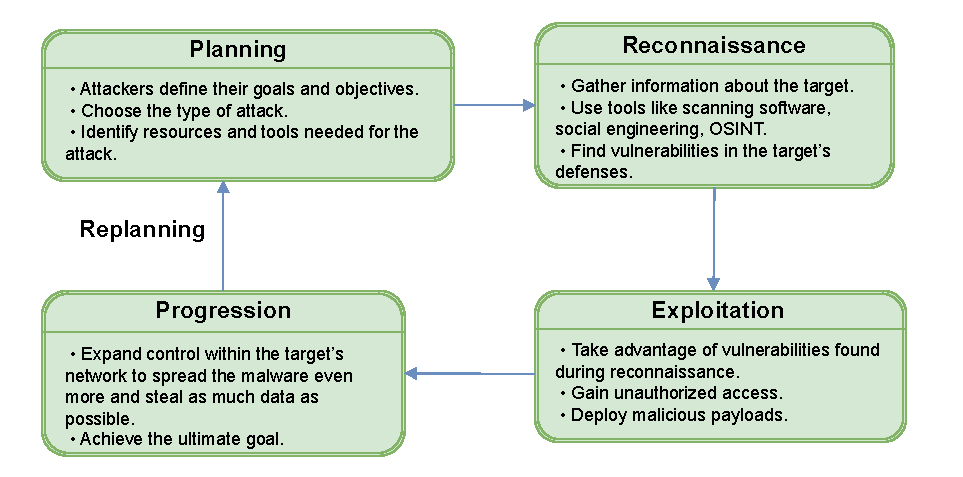
\includegraphics[width=0.9\textwidth]{Chapters/Diagram/Introduction/attack.drawio.pdf}
\end{center}

\vspace{0.35cm}
\section{Reasons for Poor Security}
\begin{prettyBox}{Reasons}{myblue}
\begin{itemize}
    \item \textbf{Insufficient Budget}: Approximately \(\frac{1}{4}\) of issues arise due to inadequate funding for cybersecurity initiatives and personnel.
    \item \textbf{Unqualified Personnel}: A lack of skilled and properly trained cybersecurity professionals.
    \item \textbf{Poor Administration}: Inefficient management and lack of synchronization in security policies and practices.
\end{itemize}
\end{prettyBox}

\vspace{0.35cm}

\section{Impacts of a Cyberattack}
\begin{prettyBox}{Impacts}{myblue}
\begin{itemize}
    \item \textbf{Data Breach}: Unauthorized access to sensitive client or organizational data. This may include\\ encrypting data for ransom (ransomware), sharing confidential information, or selling it on the dark web.  
    \item \textbf{Denial of Service (DoS)}: Disrupting or halting the services of an organization, making them inaccessible to users.   
    \item \textbf{Financial Loss}: Hacking into bank accounts, demanding ransom (ransomware attacks), or causing service interruptions that result in revenue loss.  
    \item \textbf{Damage to Reputation}: Eroding client trust or tarnishing someone's reputation by exposing compromised or sensitive data.  
    \item \textbf{Loss of Clients}: Organizations may lose clients due to the exposure of sensitive information, compromised systems, server outages, and interruptions in services.  
\end{itemize}
\end{prettyBox}

\newpage

\section{Information System}
\begin{prettyBox}{Definition}{myblue}
A set of active applications, services, and other components that allow for the management of informations.
Vulnerabilities can affect all components of the information system (IS).  
\end{prettyBox}

\section{Responses to Cyberattacks}
\begin{prettyBox}{Responses}{myblue}
\begin{itemize}
    \item \textbf{Reduce the Impact}: Taking measures to minimize the damage caused by the cyberattack, such as isolating affected systems, restoring backups, or limiting access.  
    \item \textbf{Accept the Risk}: The least effective response, where no action is taken to counter the attack. This could include surrendering to attackers’ demands, such as paying a ransom.  
    \item \textbf{Refuse or Resolve the Risk}: Actively countering the attack by refusing to comply with attackers and taking corrective actions to fix vulnerabilities or breaches.  
    \item \textbf{Transfer the Responsibility}: Shifting the burden of dealing with the cyberattack to a third party, such as an insurance provider or a managed cybersecurity service.  
\end{itemize}
\end{prettyBox}

\vspace{0.5cm}

\section{Steps For Protection (Deming's Wheel)}
\begin{prettyBox}{PDCA}{myblue}
    The PDCA (Plan-Do-Check-Act) cycle is a continuous improvement process widely used in
cybersecurity to ensure effective protection and adapt to evolving threats. Below are the four key steps:

    \begin{itemize}
        \item \textbf{\textcolor{green}{P}lan}: Identify goals, assess risks, and develop strategies to strengthen cybersecurity.
        \item \textbf{\textcolor{green}{D}o}: Implement the cybersecurity measures, like deploying firewalls and training staff.
        \item \textbf{\textcolor{green}{C}heck}: Monitor and evaluate the effectiveness of security measures through audits and testing.
        \item \textbf{\textcolor{green}{A}ct}: Address weaknesses and refine security measures to adapt to new threats.
    \end{itemize}
\end{prettyBox}

\begin{center}
    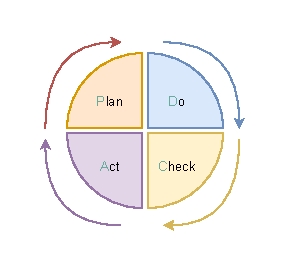
\includegraphics[width=0.5\textwidth]{Chapters/Diagram/Introduction/pdca.drawio.pdf}
\end{center}

\newpage
\section{Objectives Of Cybersecurity}
\begin{prettyBox}{Objectives}{myblue}
\begin{itemize}
\item \textbf{Confidentiality:} Ensuring that information is accessible only
to authorized individuals or systems.
\item \textbf{Integrity:} Protecting information from being altered or tampered
with by unauthorized parties.   
\item \textbf{Availability:} Ensuring that information and resources are 
accessible when needed by authorized users.    
\item \textbf{Accountability:} Tracking and attributing actions to specific
individuals or systems to ensure responsibility.    
\item \textbf{Non-Repudiation:} Preventing individuals or systems from
denying their actions or commitments.
\end{itemize}
\end{prettyBox}

\vspace{0.75cm}

\section{Domain Of Cybersecurity}
\begin{prettyBox}{Domain}{myblue}
\begin{itemize}
\item \textbf{Physical Security:} Protecting physical assets (e.g., servers,
devices, and facilities) from unauthorized access, theft, or damage.
\item \textbf{OS Security:} Securing operating systems by implementing measures
like access controls, patches, and malware protection.
\item \textbf{Logical Security:} Safeguarding data and systems through 
software-based controls like encryption, firewalls, and authentication.
\item \textbf{Application Security:} Ensuring that applications are secure by
identifying and fixing vulnerabilities during development and deployment.
\item \textbf{Telecommunication Security:} Protecting communication systems
(e.g., networks, phones, and \\internet) from interception, eavesdropping, or 
attacks.
\end{itemize}
\end{prettyBox}

\vspace{0.75cm}

\section{Transmission Security}
\begin{prettyBox}{Transmission Security}{myblue}
\begin{itemize}
    \item Only the intended recipient can access the message.
    \item Verify the identity of both the sender and the receiver.
    \item Ensure that the message sent and the message received are identical.
    \item Provide proof that the message was successfully sent and received.
\end{itemize}
\end{prettyBox}

\vspace{0.75cm}
\section{Identification \& Authentication}
\begin{prettyBox}{Identification \& Authentication}{myblue}
\begin{itemize}
    \item \textbf{Identification:} The process of claiming an identity (e.g., providing a username or email address).
    \item \textbf{Authentication:} The process of verifying the claimed identity (e.g., using a password, biometrics, or a one-time code).
    \item \textbf{Example - Two-Factor Authentication (2FA):} 
    \begin{itemize}
        \item \textbf{Step 1 - Identification:} Provide a username or email.
        \item \textbf{Step 2 - Authentication:} 
        \begin{itemize}
            \item \textbf{First Factor:} Provide a password.
            \item \textbf{Second Factor:} Input the code that was sent to your email or phone number
        \end{itemize}
    \end{itemize}
\end{itemize}
\end{prettyBox}

\vspace{0.75cm}

\section{The Risks of Network Security}
\begin{prettyBox}{The Risks}{myblue}
\begin{itemize}
    \item Theft of passwords and personal data.
    \item Insertion of malware and viruses.
    \item Spoofing of source addresses.
    \item Violation of data integrity.
    \item Denial of Service (DoS) attacks.
\end{itemize}
\end{prettyBox}

\vspace{0.75cm}

\section{Objectives of Attacks}
\begin{prettyBox}{Objectives}{myblue}
\begin{itemize}
    \item Misinforming.
    \item Denying access to a resource.
    \item Taking control of a resource.
    \item Stealing data present in the system.
    \item Using the system as a relay.
    \item Creating a botnet network (zombies).
\end{itemize}
\end{prettyBox}

\newpage

\section{Attacks}
\begin{prettyBox}{Attacks}{myblue}
\begin{itemize}
\item \textbf{DOS (Denial of Service):} An attack that overwhelms a system, 
making it unavailable to users by flooding it with excessive requests.
\item \textbf{DDOS (Distributed Denial of Service):} A more advanced form of 
DOS where multiple systems (often compromised) are used to flood a target, 
making it harder to mitigate.
\item \textbf{MITM (Man-in-the-Middle):} An attack where an attacker 
intercepts and potentially alters communication between two parties without 
their knowledge.
\item \textbf{IP Spoofing:} An attack where an attacker disguises their IP 
address to impersonate another system, often to gain unauthorized access or 
launch further attacks.
\item \textbf{DNS Spoofing/Poisoning:} An attack where an attacker corrupts 
DNS records to redirect users to malicious websites instead of legitimate ones.
\item \textbf{Smurf Attack:} A type of DOS attack where the attacker sends 
spoofed ICMP packets to broadcast addresses, causing multiple systems to 
respond and overwhelm the target.
\item \textbf{Port Scan:} An attack where an attacker scans a system for open 
ports to identify potential vulnerabilities or services to exploit.
\item \textbf{Phishing:} A social engineering attack where attackers trick 
users into revealing sensitive information (e.g., passwords) by pretending to be a 
trusted entity.
\item \textbf{Hoax:} A false message or warning designed to deceive users, 
often causing unnecessary panic or spreading misinformation.
\item \textbf{Bot or Zombie:} A compromised computer controlled by an attacker, often used to carry out malicious activities like DDOS attacks or spam distribution.
\item \textbf{Backdoor:} A hidden method of bypassing normal authentication or 
security mechanisms, often left by attackers to regain access to a system.
\end{itemize}
\end{prettyBox}

\vspace{0.75cm}


\section{Types of Malware}
\begin{prettyBox}{Types}{myblue}
\begin{itemize}
    \item \textbf{Worm:} A self-replicating malware that spreads across
networks without user action. It consumes system resources and can deliver 
malicious payloads.
    \item \textbf{Spyware:} Software that secretly monitors user activity, 
collecting personal data such as passwords, browsing habits, or financial 
information.
    \item \textbf{Rootkit:} A hidden malware that provides hackers deep access 
to a system while avoiding detection, often modifying system files.
    \item \textbf{Logic Bomb:} Malicious code hidden inside a program that 
activates under specific conditions, such as a certain date or user action.
\end{itemize}
\end{prettyBox}

\vspace{0.75cm}

\section{Types Of Hackers}
\begin{prettyBox}{Types}{myblue}
\begin{itemize}
    \item \textbf{Anonymous:} Hackers who act without revealing their identity, often working individually or in loosely connected groups.
    \item \textbf{Cyber-Indigned:} Activist hackers (hacktivists) who attack systems to protest or promote a political, social, or ideological cause.
    \item \textbf{Cyber-Armed:} Hackers who possess advanced skills and tools, often working for governments or military operations to conduct cyber warfare.
    \item \textbf{Cyber-Criminal:} Hackers who engage in illegal activities for financial gain, such as stealing data, fraud, or ransomware attacks.
\end{itemize}
\end{prettyBox}

\vspace{0.75cm}

\section{How To Protect Ourselves}
\begin{prettyBox}{Protection}{myblue}
\begin{itemize}
    \item \textbf{Antivirus:} Software that detects, prevents, and removes 
malware by scanning files and monitoring system behavior.
    \item \textbf{IDS/IPS (Intrusion Detection/Prevention System):} Security 
tools that monitor network traffic to detect (IDS) or block (IPS) suspicious 
activity.
    \item \textbf{OS Firewall:} A built-in security feature in operating 
systems that filters incoming and outgoing network traffic to prevent 
unauthorized access.
    \item \textbf{Anti-spam:} Software that filters unwanted emails, blocking 
phishing attempts, scams, and malware hidden in messages.
\end{itemize}
\end{prettyBox}

